
\section{Collaboration Efficiency}

To quantify the benefits of transitioning from a sequential, single-arm architecture to a multithreaded, dual-arm collaborative cell, several Key Performance Indicators (KPIs) were established. The primary metrics evaluated include total cycle time, parallel execution efficiency, and the reliability of the handover state machine.

\subsection{Execution Timing and Throughput}

Throughput and cycle time were measured by executing a standardized assembly sequence, distributed between the AR4 and ABB reachable workspaces. The system was benchmarked under two operational paradigms: strictly sequential execution (where only one arm moves at any given time) and the implemented parallel execution framework. The performance metrics collected include:


\begin{itemize}
    \item \textbf{Total Assembly Time ($T_{total}$):} The absolute time from the initialization of the first pick command to the completion of the final place command.
    \item \textbf{Parallel Utilization Rate ($U_p$):} The percentage of the total assembly time where both manipulators were in simultaneous motion.
    \item \textbf{Arm Starvation/Idle Time ($T_{idle}$):} The cumulative time an arm spent waiting for the other to clear a shared zone or complete a handover.
\end{itemize}


\begin{table}[H]
    \centering
    \caption{Cycle Time Comparison: Sequential vs. Parallel Execution}
    \label{tab:cycle_time_comparison}
    \begin{tabular}{lccc}
        \toprule
        \textbf{Metric} & \textbf{Sequential Mode} & \textbf{Parallel Mode} & \textbf{Improvement (\%)} \\
        \midrule
        Total Assembly Time (s) & 74.8 & 40.0 & 46.5\% \\
        AR4 Active Time (s)     & 37.0 & 35.2 & - \\
        ABB Active Time (s)     & 33.1 & 33.6 & - \\
        Total Idle Time (s)     & 79.5 & 11.1 & 86.0\% \\
        \bottomrule
    \end{tabular}
\end{table}

\begin{figure}[H]
    \centering
    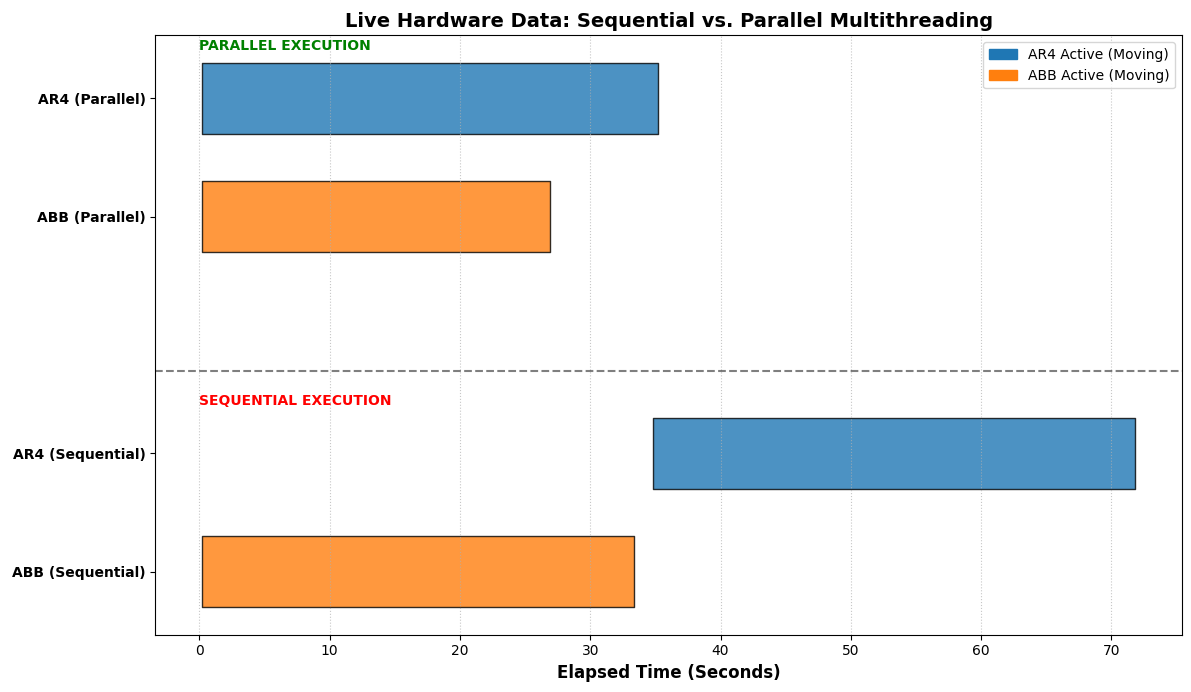
\includegraphics[width=1\textwidth]{figures/chapter7/collab_efficiency/Sequential Vs Parallel.png}
    \caption{Comparing sequential logic against the parallel execution framework.}
    \label{fig:gantt_chart}
\end{figure}

\subsection{Sequential and Hybrid MTC Execution Comparison}

A focused cycle-time comparison was conducted between the conventional sequential handover implementation and the Hybrid MoveIt Task Constructor (MTC) implementation. In the sequential approach, each AR4 and ABB operation was executed individually, with the following operation starting only after the previous operation had completed. In comparison, the Hybrid MTC approach coordinated the complete pick, handover, placement, and return sequence through a unified task pipeline.

The sequential handover cycle was divided into seven individual execution phases, while the Hybrid MTC implementation was represented by three main functional phases. The measured durations are presented in Table~\ref{tab:sequential_mtc_comparison}.

\begin{table}[H]
    \centering
    \caption{Execution Time Comparison Between Sequential and Hybrid MTC Approaches}
    \label{tab:sequential_mtc_comparison}
    \begin{tabular}{lcc}
        \toprule
        \textbf{Execution Phase} & \textbf{Approach} & \textbf{Duration (s)} \\
        \midrule
        AR4 Pick Phase & Sequential & 13.297 \\
        AR4 Handover Approach & Sequential & 4.561 \\
        ABB Handover Synchronization & Sequential & 7.991 \\
        AR4 Post-Handover Retraction & Sequential & 3.231 \\
        AR4 Return to Home & Sequential & 4.966 \\
        ABB Transfer to Placement & Sequential & 5.900 \\
        ABB Return to Home & Sequential & 4.680 \\
        \midrule
        \textbf{Total Sequential Time} & \textbf{Sequential} & \textbf{44.626} \\
        \midrule
        Object Pick and Handover & Hybrid MTC & 18.894 \\
        Waiting for Grasp-Point Generation & Hybrid MTC & 0.017 \\
        Object Placement and Return Home & Hybrid MTC & 17.180 \\
        \midrule
        \textbf{Total Hybrid MTC Time} & \textbf{Hybrid MTC} & \textbf{36.091} \\
        \bottomrule
    \end{tabular}
\end{table}

The Hybrid MTC approach reduced the total cycle time from 44.626~s to 36.091~s. This corresponds to an absolute reduction of 8.535~s and a cycle-time improvement of approximately 19.1\%, calculated as:

\begin{equation}
    \text{Cycle-Time Improvement}
    =
    \frac{44.626 - 36.091}{44.626}
    \times 100
    =
    19.1\%
\end{equation}

The Hybrid MTC implementation therefore completed the full handover cycle approximately 1.23 times faster than the sequential implementation. The improvement resulted from combining the manipulation stages into a coordinated task pipeline and reducing the waiting periods introduced by individually triggered sequential actions.

\begin{figure}[H]
    \centering
    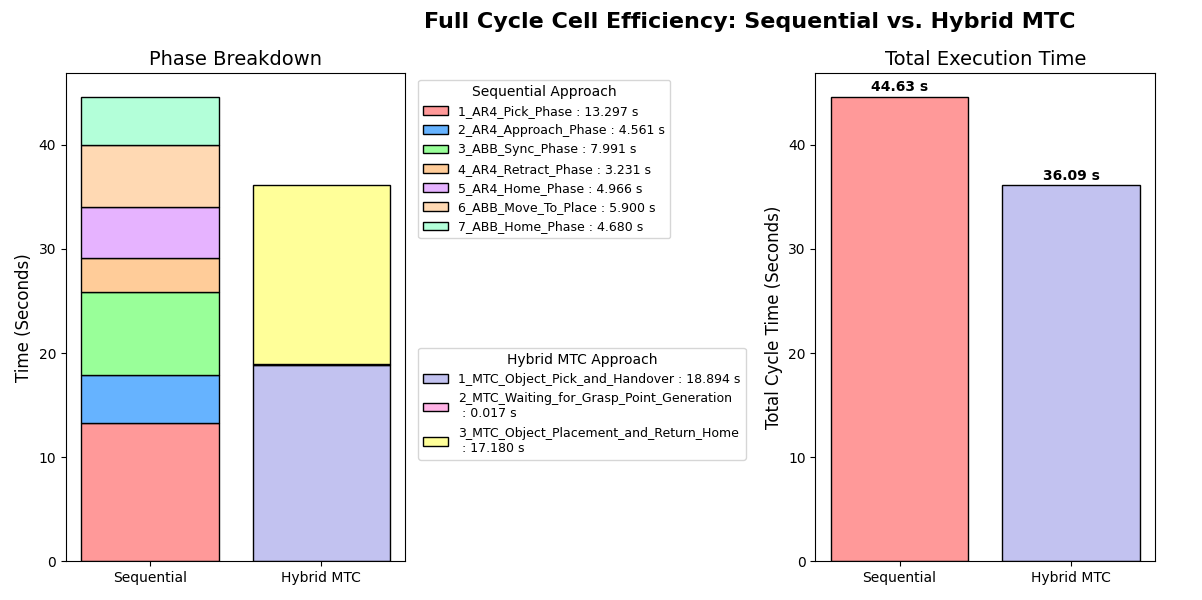
\includegraphics[width=1\textwidth]{figures/chapter7/collab_efficiency/handover_comparison_chart.png}
    \caption{Full-cycle execution-time comparison between the sequential and Hybrid MTC handover approaches.}
    \label{fig:sequential_hybrid_mtc_comparison}
\end{figure}

Figure~\ref{fig:sequential_hybrid_mtc_comparison} presents both the phase-level execution breakdown and the total cycle time of the two approaches. Although the Hybrid MTC approach contains fewer reported phases, each phase represents a broader coordinated part of the handover workflow. Therefore, the comparison should primarily be interpreted using the complete cycle duration rather than by directly comparing individual phases between the two implementations.



\subsection{Handover Phase Execution Metrics}

The collaborative handover process is mechanically and logically complex, requiring precise dynamic orientation, particularly when dealing with asymmetric components such as Z-shape bricks. The handover state machine was analyzed based on its computational overhead and temporal efficiency during a successful execution sequence.

The handover was decomposed into three principal functional phases to remain consistent with the timing boundaries reported by the Hybrid MoveIt Task Constructor (MTC) implementation. Each principal phase contains internal computational and physical operations. The performance metrics collected include:

\begin{itemize}
    \item \textbf{MTC Planning, AR4 Pick, and Transport to Handover Pose:} This phase includes the MTC computation time required by the pipeline planner to calculate the synchronized Cartesian motion and the dynamic presentation yaw. It also includes the physical execution of the AR4 object-picking motion and transport to the predefined handover pose.
    \item \textbf{ABB Grasp-Point Generation at Handover Pose:} After the AR4 reaches and maintains the handover pose, the grasping model analyzes the presented object and generates a valid grasp point for the ABB manipulator. The measured grasp-point generation time was 17~ms.
    \item \textbf{ABB Spatial Approach, Transfer, Placement, and Safe Retraction:} This phase includes the spatial approach time required for the ABB to converge with the AR4 at the predefined handover coordinate. It also includes the internal ROS 2 gripper handshake, object transfer, safe retraction of both manipulators, ABB placement, and the final return-home motion.
\end{itemize}

The MTC computation time is included within the first principal phase. Grasp-point generation is reported as the second phase because it occurs after the AR4 reaches the handover pose. The ABB spatial approach, gripper synchronization, object transfer, safe retraction, placement, and return-home operations are grouped within the third phase. Hardware synchronization is therefore treated as an internal operation rather than as a separate main phase.

\begin{table}[H]
    \centering
    \caption{Temporal Execution Metrics for Collaborative Handover Sequence}
    \label{tab:handover_metrics}
    \begin{tabular}{lcc}
        \toprule
        \textbf{Handover Phase} & \textbf{Duration (s)} & \textbf{\% of Total Exchange} \\
        \midrule
        MTC Planning, AR4 Pick, and Handover Transport & 18.894 & 52.35\% \\
        ABB Grasp-Point Generation & 0.017 & 0.05\% \\
        ABB Approach, Transfer, Placement, and Retraction & 17.180 & 47.60\% \\
        \midrule
        \textbf{Total Exchange Time} & \textbf{36.091} & \textbf{100.0\%} \\
        \bottomrule
    \end{tabular}
\end{table}

\begin{figure}[H]
    \centering
    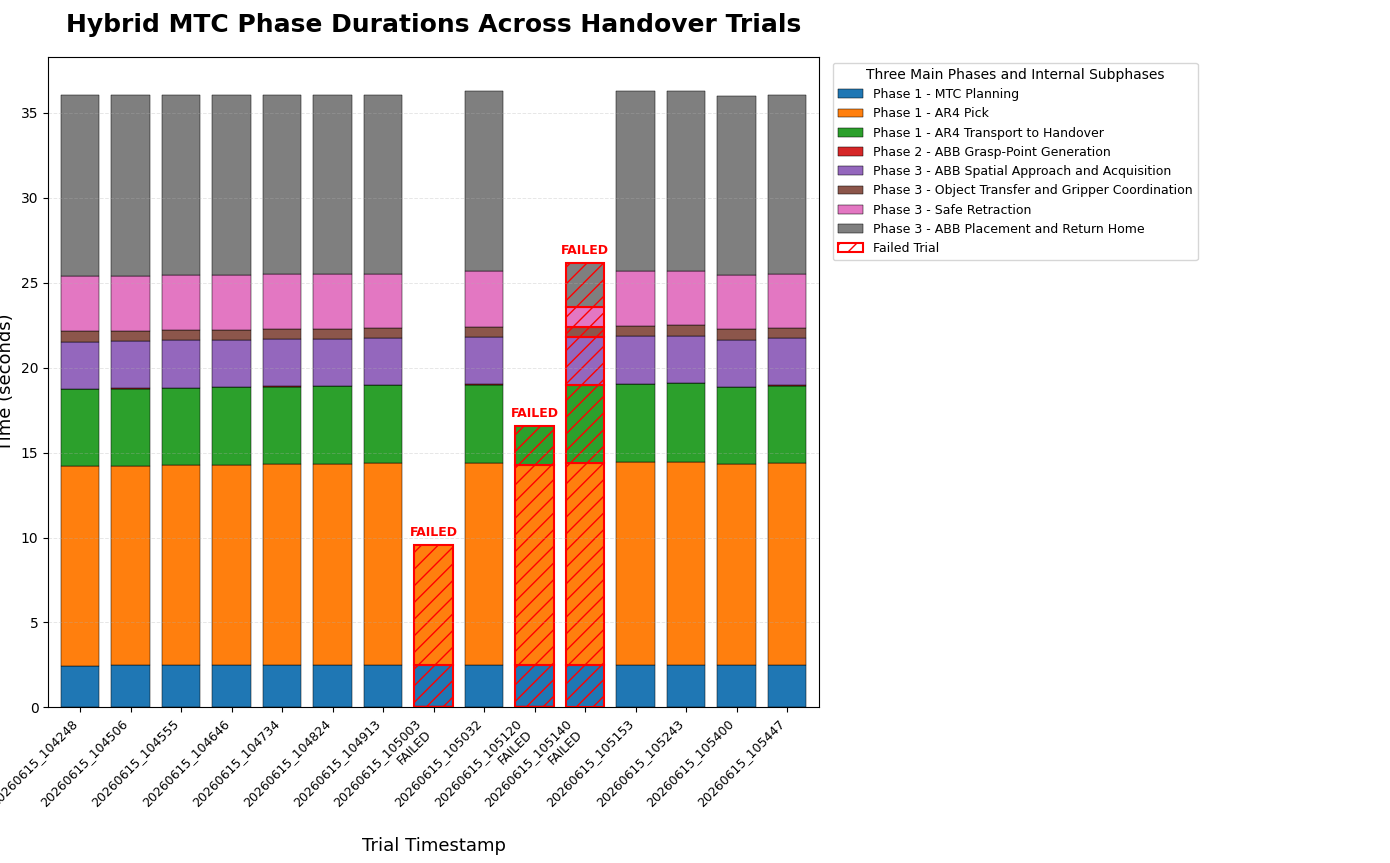
\includegraphics[width=1\textwidth]{figures/chapter7/collab_efficiency/thesis_handover_performance.png}
    \caption{Collaborative Handover Phase Durations.}
\end{figure}

\subsection{Handover Reliability}

The reliability of the collaborative handover process was evaluated across 15 experimental trials. A trial was considered successful when the complete handover sequence was executed, including MTC planning, object acquisition by the AR4, movement to the handover pose, valid grasp-point generation for the ABB, synchronized object transfer, final placement, and safe retraction of both manipulators.

Out of the 15 experimental trials, 12 trials successfully completed the full handover process, while three trials failed at different stages of the sequence. Therefore, the collaborative handover system achieved an overall success rate of 80.0\%.

\begin{table}[H]
    \centering
    \caption{Collaborative Handover Reliability Results}
    \label{tab:handover_reliability}
    \begin{tabular}{lc}
        \toprule
        \textbf{Reliability Metric} & \textbf{Result} \\
        \midrule
        Total Trials & 15 \\
        Successful Trials & 12 \\
        Failed Trials & 3 \\
        \textbf{Success Rate} & \textbf{80.0\%} \\
        \bottomrule
    \end{tabular}
\end{table}

The three failed trials occurred at different stages of the handover process. In the first failed trial, the AR4 was unable to grasp the object during Phase~1. In the second failed trial, the AR4 successfully grasped the object but failed to reach the predefined handover pose during the transport stage of Phase~1. In the third failed trial, the ABB completed the handover but failed to reach the pre-place pose during Phase~3 because its gripper did not close securely after receiving the object.

The failed trials were included in the reliability calculation but were excluded from the average temporal execution metrics because they did not complete the full handover sequence.

\begin{figure}[H]
    \centering
    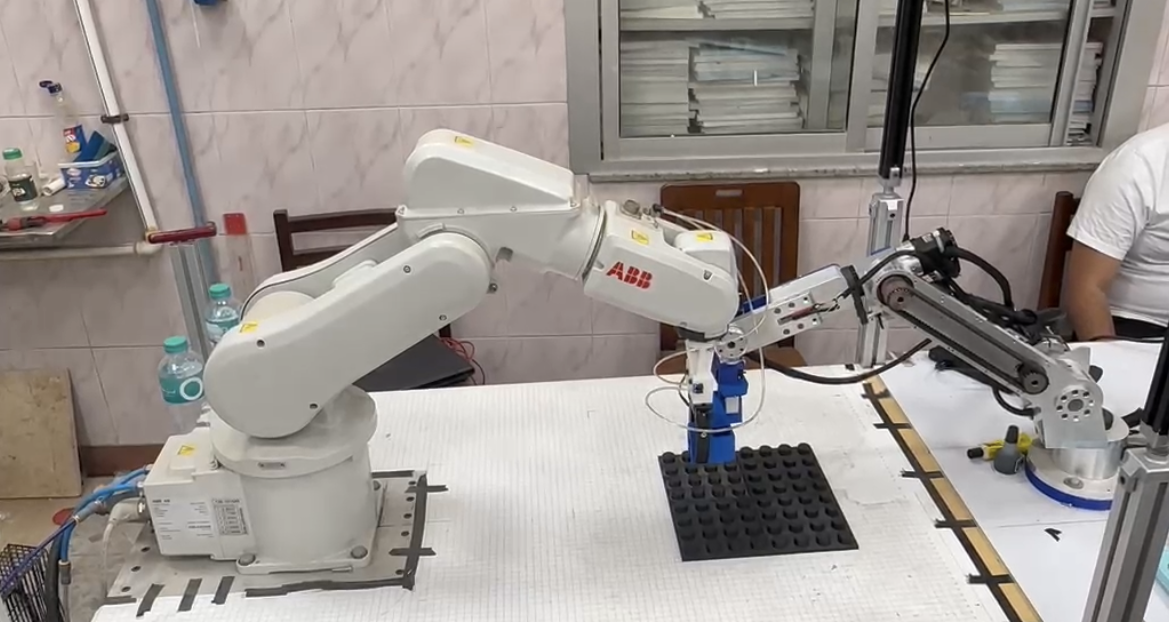
\includegraphics[width=0.6\textwidth]{figures/chapter7/collab_efficiency/physical_handover.png}
    \caption{Physical execution of the handover sequence.}
    \label{fig:physical_handover}
\end{figure}

\clearpage
